\documentclass{standalone}
\usepackage[utf8]{inputenc}
\usepackage[T1]{fontenc}
\usepackage{graphicx}
\usepackage{amsmath}
\usepackage[american,siunitx]{circuitikz}
\usetikzlibrary{arrows,shapes,calc,positioning}
\usepackage{tikzsymbols}

    
\begin{document}
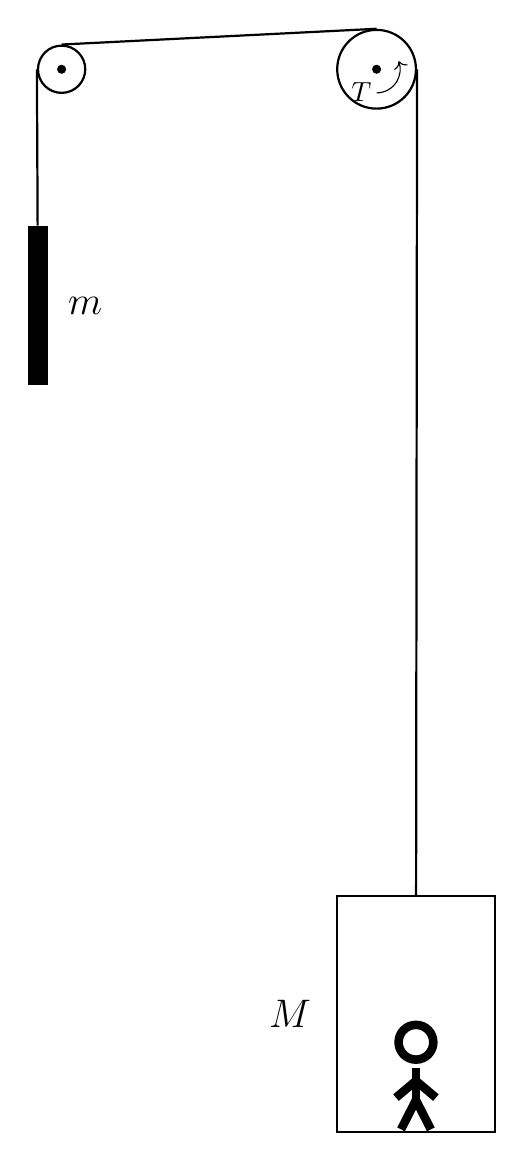
\begin{tikzpicture}
  \node[circle, draw, thick, minimum width=1cm] (pulley) at (0,0) {};
  \node[circle, draw, fill, black, minimum width=1mm, inner sep=0pt] (axle) at (0,0) {};
  \begin{scope}[rotate=-90]
  \draw[->] (3mm,0 ) arc[start angle=0, end angle=110, radius=3mm] node[pos=0.1,left] {$T$};
  \end{scope}

  \node[circle, draw, thick, minimum width=6mm] (idler) at (-4,0) {};
  \node[circle, draw, fill, black, minimum width=1mm, inner sep=0pt] at (-4,0) {};

  \node[draw, thick, minimum height=3cm, minimum width=2cm] (cabin) at (0.5,-12) {};
  \node at (0.5, -12.8) {\Strichmaxerl[6][40][-40]};
  \node[draw, thick, fill, minimum height=2cm, minimum width=2mm] (counterw) at (-4.3,-3) {};
  \node[right of=counterw, node distance=6mm] {\Large $m$};
  \node[left of=cabin, node distance=16mm] {\Large $M$};
  
  \draw[thick] (cabin) -- (pulley.east);
  \draw[thick] (pulley.north) -- (idler.north);
  \draw[thick] (counterw) -- (idler.west);
  
  
\end{tikzpicture}
\end{document}
